\section{Modeling and Evaluation Protocol}\label{sec:protocol}

Every number reported in this paper and the next is produced by a single, shared training-and-evaluation harness applied identically to all four modeled datasets (BankSim, IBM~AML, SAP~W\"urzburg, and the in-house synth\_erp corpus). This section specifies that harness precisely enough to be reproduced: the learner and its fixed hyperparameter defaults, the two mutually exclusive imbalance mechanisms, the chronological splitting rule (including a partition-aware variant required by one dataset's own construction), the threshold-freezing procedure, the metric suite, and the attribution method. The harness is deliberately narrow — one function, one set of rules, applied the same way whether the feature set under test is a lean eight-column ordinary baseline or a ninety-nine-column champion bundle. Section~\ref{sec:ablation} then uses this exact protocol, unmodified, to answer the paper's central question.

\subsection{Model family: gradient-boosted trees, histogram method}
Every arm in this paper is an XGBoost classifier \cite{chen2016xgboost} with \texttt{tree\_method="hist"}, trained for up to 500 boosting rounds with early stopping after 40 rounds without validation-PR-AUC improvement. A single locked default configuration anchors every comparison: \texttt{max\_depth=6}, \texttt{learning\_rate=0.05}, \texttt{subsample=0.8}, \texttt{colsample\_bytree=0.8}, \texttt{min\_child\_weight=5}, \texttt{reg\_lambda=1.0}, \texttt{reg\_alpha=0.0}. Where a light random hyperparameter search (20 sampled configurations, scored on validation PR-AUC only) is run for a dataset's final champion, this default configuration is always included as candidate zero, so a tuned model can never underperform the untuned baseline on the selection metric it will be judged by. The search is automatically skipped when a split's validation-set fraud count is judged too small to support it without overfitting hyperparameters to a handful of positives — the guard that fires for SAP W\"urzburg (19 validation frauds), discussed further in \S\ref{sec:ablation-stats}.

\subsection{One imbalance mechanism, never two}
Fraud rates in the four datasets range from roughly 0.1\% to 1.2\% of rows. The harness offers exactly two ways to counteract this, selected per run and recorded in every saved artifact, and never combined: (i) \emph{class weighting}, XGBoost's native \texttt{scale\_pos\_weight} set to the train-split negative-to-positive ratio, and (ii) an \emph{alpha-free focal-loss} objective \cite{lin2017focal}, implemented as a custom XGBoost objective with a closed-form gradient and a central-finite-difference Hessian, trained with \texttt{scale\_pos\_weight=1.0}. The focal variant is deliberately \emph{unweighted} (symmetric, no per-class $\alpha$ term): the common alpha-balanced formulation of focal loss secretly reintroduces a class-prior weight, which would silently stack a second imbalance mechanism on top of the first — precisely the failure mode this protocol is built to exclude. Because a focal objective returns a raw margin rather than a probability, every downstream consumer (threshold tuning, PR-AUC, TreeSHAP) is written to accept either representation, applying a sigmoid only where a probability is actually required. Synthetic minority oversampling (SMOTE) is excluded from the harness entirely, on the grounds that an interpolated point between two topology vectors — half a cycle, a fractional fan-in count — has no physical meaning in a transaction graph.

Which mechanism wins is decided the same way as any other hyperparameter: on validation-split PR-AUC, never on the test split. Per \texttt{final\_champions.json}, focal loss wins the selection on three of the four datasets — BankSim (validation PR-AUC mean $0.9515$ vs.\ $0.94891$ for class weighting), SAP W\"urzburg ($0.35619$ vs.\ $0.28875$, though this particular selection is separately flagged \texttt{reliable:\ false} owing to the small-sample guard above), and synth\_erp ($0.85066$ vs.\ $0.84866$). IBM~AML is the exception, and an instructive one: both mechanisms reach a validation PR-AUC of exactly $1.0$ with zero variance across three seeds, so the "winner" (class weighting, by tie-break) is not really a comparison at all — an early symptom of the baseline-saturation story developed in \S\ref{sec:ablation}.

\subsection{Chronological splitting, including a partition-aware variant}
Every split is a 60/20/20 train/validation/test partition by transaction timestamp, and rows are never shuffled: the training set is defined as the earliest 60\% of transactions by time, validation the next 20\%, and test the final, strictly future 20\%. For most datasets this is a single global quantile cut on the timestamp axis. SAP W\"urzburg is the exception: its raw export orders postings by \texttt{run\_id} (audit run), and each run is internally fraud-first-then-clean, so a global time cut would strand an entire zero-fraud run inside the validation split. The harness therefore applies a \emph{partition-aware} variant for this dataset — the same 60/20/20 chronological rule, but computed independently within each \texttt{run\_id} and concatenated, so every run contributes its own early rows to train and its own late rows to test. This is still a strictly chronological, never-shuffled split; only the unit over which the time cut is computed changes.

Two independent partition-aware splits of SAP W\"urzburg appear in this project's own committed artifacts, and they differ by a small margin that we flag rather than silently reconcile. The ablation run (\texttt{ablation.json}) reports train/val/test sizes of $120{,}411$/$40{,}137$/$40{,}139$; the later final-champion run (\texttt{final\_champions.json}) reports $120{,}341$/$40{,}114$/$40{,}116$ — a difference of 116 rows, or about 0.06\% of the dataset. Both runs use the identical partition-aware algorithm described above, so the discrepancy is not a change in splitting logic; it most plausibly reflects a small difference in row count between two separate ETL/feature-build passes of the same source file. We did not further trace its exact origin. Every SAP W\"urzburg figure in this paper is therefore attributed to the specific source file it was read from, and the two split-size counts should not be added, averaged, or treated as interchangeable.

\subsection{Threshold tuning: frozen before the test set is touched}
XGBoost outputs a continuous score; converting it into a binary alert requires a cutoff, and an arbitrary $0.5$ is never used. Instead, the harness scans the validation-set precision--recall curve and selects the threshold that maximizes F1 on validation data alone. That threshold is then frozen and applied, unmodified, to the held-out test split — the test set never participates in threshold selection. In practice the chosen threshold varies considerably by feature set even within one dataset (for BankSim, $0.9673$ for the ordinary baseline vs.\ $0.9549$ for the topology-augmented model; \texttt{ablation.json}), underscoring why a single fixed cutoff across models would confound feature-set comparisons with cutoff artifacts.

\subsection{Primary and operational metrics}
PR-AUC (average precision) is the primary metric throughout this paper and the sole metric used for model and mechanism selection; it is never selected on F1-at-a-fixed-threshold, which would hide the cutoff problem the previous subsection exists to solve. ROC-AUC is reported alongside it but never relied upon: on data this skewed (fraud rates of 0.1--1.2\%), ROC-AUC is inflated by the overwhelming volume of easy true negatives and routinely exceeds 0.99 even for models with weak operational precision (Table~\ref{tab:ablation-arms}, SAP W\"urzburg's baseline arm: ROC-AUC $0.991$ against a PR-AUC of only $0.155$). Because an audit team reviews a bounded daily list of alerts rather than a probability distribution \cite{vasarhelyi2012acceptance}, every evaluation also reports precision@$k$ and recall@$k$ for $k \in \{50, 100, 500, 1000\}$ — of the top-$k$ highest-scored transactions, what fraction are confirmed fraud, and what fraction of all fraud that budget would catch. F1 at the frozen threshold is reported for completeness but, as noted, is never a selection criterion.

\subsection{Attribution: exact TreeSHAP in margin space}
Every reported feature attribution is computed via XGBoost's native \texttt{pred\_contribs} interface rather than a sampling-based SHAP approximation. With \texttt{pred\_contribs=True}, the booster runs the exact TreeSHAP recursion \cite{lundberg2017unified,lundberg2020local} — algorithmically identical to the \texttt{shap} package's \texttt{TreeExplainer} for tree ensembles — as a pure traversal of the fitted trees, returning one signed contribution per feature per row plus a base value, additive in margin (log-odds) space. This is exact, not approximate, and its cost is a fixed function of tree structure rather than a sampling budget. It is also, crucially, agnostic to which of the two imbalance mechanisms trained the model: because a focal-loss booster is still an ordinary ensemble of regression trees whose leaves were fit against a focal gradient, the same margin-space traversal applies unchanged, with only the final sigmoid step (used only where a probability is required, e.g.\ threshold comparisons) built to know which mechanism produced the raw score. This gives every model in this paper's evaluation suite — baseline, topology-augmented, and the final TGN-plus-topology champion alike — an exact, common explanation mechanism, discussed further in the explainability sections that follow.

\section{The Ablation: Does Topology Add Value?}\label{sec:ablation}

The protocol of \S\ref{sec:protocol} exists to answer one question honestly: \emph{do graph-topology features add predictive value over a strong ordinary-transaction baseline, measured without leakage?} This section reports that answer as a seven-arm ablation run identically, with identical splits, model family, and imbalance-mechanism selection, on each of the four modeled datasets. We commit, per the project's own methodology rules, to reporting the result exactly as measured — including where it is negative, where it is uninformative, and where it rests on too few positive examples to trust.

\subsection{The seven-arm decomposition}
A naive ablation — ordinary features alone vs.\ ordinary-plus-topology — is not sufficient here for two reasons uncovered during this project's own earlier probing. First, on a dataset whose ordinary-only baseline is already close to saturated (IBM~AML: baseline PR-AUC $0.990$), a marginal comparison against the full model has almost no headroom left to measure, whatever the true value of topology. Second, several of the project's topology detectors are not, in fact, amount-blind: the lapping detectors (\texttt{lap\_in\_payers}, \texttt{lap\_in\_recur}, \texttt{lap\_out\_payees}, \texttt{lap\_out\_recur}) and the cycle amount-conservation ratio (\texttt{cycle\_amount\_ratio}) are derived in part from transaction amounts, so a topology arm that includes them can re-smuggle the amount signal into what is presented as a "structural" result. Of the thirteen topology features produced by the engine, the feature manifests confirm this split is exact and identical across all four datasets: eight are pure structure (\texttt{in\_cycle}, \texttt{cycle\_length}, \texttt{in\_cycle\_ge3}, \texttt{cycle\_time\_span}, \texttt{fan\_in}, \texttt{fan\_out}, \texttt{dest\_in\_degree}, \texttt{src\_out\_degree}), and five are amount-derived (the four lapping features plus \texttt{cycle\_amount\_ratio}).

The ablation therefore trains seven arms per dataset, all under the identical protocol of \S\ref{sec:protocol}: (1) \textbf{Baseline} — ordinary transaction features only; (2) \textbf{+Topology} — baseline plus all thirteen topology features, amount-derived ones included; (3) \textbf{+Structure} — baseline plus only the eight pure-structure features; (4) \textbf{Amount-blind baseline} — the ordinary feature set with every amount-derived column (log-amount, amount z-scores, prior amount means, \ldots) removed; (5) \textbf{Amount-blind~+~Topology}; (6) \textbf{Amount-blind~+~Structure}; and (7) \textbf{Topology-only} — the thirteen topology features with no ordinary features at all. Only arms (1) and (2) are persisted as deployable model artifacts; the remaining five exist purely to decompose \emph{why} any observed lift occurs.

From these seven arms, four scalar lift statistics are computed on the test split, each isolating a different confound:
\begin{itemize}
  \item \textbf{marginal\_topology\_lift} = PR-AUC(+Topology) $-$ PR-AUC(Baseline) — the headline number, but contaminated by amount-derived topology on a full-featured model;
  \item \textbf{marginal\_structure\_lift} = PR-AUC(+Structure) $-$ PR-AUC(Baseline) — the honest full-model claim, restricted to pure structure;
  \item \textbf{amount\_blind\_topology\_lift} = PR-AUC(Amount-blind+Topology) $-$ PR-AUC(Amount-blind baseline) — removes the amount confound from the baseline, but still contaminated because the topology arm itself contains amount-derived columns;
  \item \textbf{amount\_blind\_structure\_lift} = PR-AUC(Amount-blind+Structure) $-$ PR-AUC(Amount-blind baseline) — the \emph{clean} test: no amount information anywhere, on either side of the comparison.
\end{itemize}
Only the last of these four is free of both confounds simultaneously, and it is the number we treat as the decisive evidence for or against the paper's thesis on each dataset.

\subsection{Results across four datasets}
Table~\ref{tab:ablation-arms} reports test-split PR-AUC for all seven arms on all four datasets, read directly from \texttt{ablation.json}. Table~\ref{tab:ablation-lifts} reports the four lift statistics derived from it. Both are single-seed (seed 42) results; the statistical status of these numbers is addressed explicitly in \S\ref{sec:ablation-stats} before any of them are interpreted causally.

\begin{table}[t]
\centering
\caption{Test-split PR-AUC (average precision) across the seven ablation arms, by dataset. B = ordinary baseline; T = all topology (incl.\ amount-derived); S = pure structure only (8 of 13 topology features); subscript $\neg a$ = amount columns removed from the ordinary set. Single seed (42); \texttt{paper/data/ablation.json}.}
\label{tab:ablation-arms}
\small
\begin{tabular}{lcccc}
\toprule
Arm & BankSim & IBM AML & SAP W. & Synth-ERP \\
\midrule
B & 0.833 & 0.990 & 0.155 & 0.163 \\
B+T & 0.931 & 1.000 & 0.046 & 0.563 \\
B+S & 0.930 & 0.998 & 0.072 & 0.566 \\
B$_{\neg a}$ & 0.634 & 0.093 & 0.049 & 0.157 \\
B$_{\neg a}$+T & 0.822 & 0.867 & 0.055 & 0.503 \\
B$_{\neg a}$+S \emph{(clean)} & 0.824 & 0.184 & 0.064 & 0.269 \\
T-only & 0.483 & 0.633 & 0.024 & 0.306 \\
\bottomrule
\end{tabular}
\end{table}

\begin{table}[t]
\centering
\caption{The four ablation lift statistics (test-split PR-AUC deltas). Positive = helps; negative = hurts. \texttt{paper/data/ablation.json}.}
\label{tab:ablation-lifts}
\small
\resizebox{\columnwidth}{!}{%
\begin{tabular}{lcccc}
\toprule
Dataset & $\Delta$Topo (full) & $\Delta$Struct (full) & $\Delta$Topo (blind) & $\Delta$Struct (blind, clean) \\
\midrule
BankSim & +0.0977 & +0.0974 & +0.1883 & +0.1899 \\
IBM AML & +0.0100 & +0.0079 & +0.7735 & +0.0905 \\
SAP W. & $-$0.1090 & $-$0.0829 & +0.0056 & +0.0153 \\
Synth-ERP & +0.4000 & +0.4031 & +0.3451 & +0.1115 \\
\bottomrule
\end{tabular}}
\end{table}

%% FIGURE TODO: grouped bar chart, one group per dataset (BankSim, IBM AML, SAP Wurzburg, Synth-ERP), four bars per group showing the four lift statistics from Table 2 (marginal-topology, marginal-structure, amount-blind-topology, amount-blind-structure), with a zero line and SAP Wurzburg's two negative bars visually distinct (e.g. hatched/red) from the three positive datasets.
\begin{figure}[t]
\centering
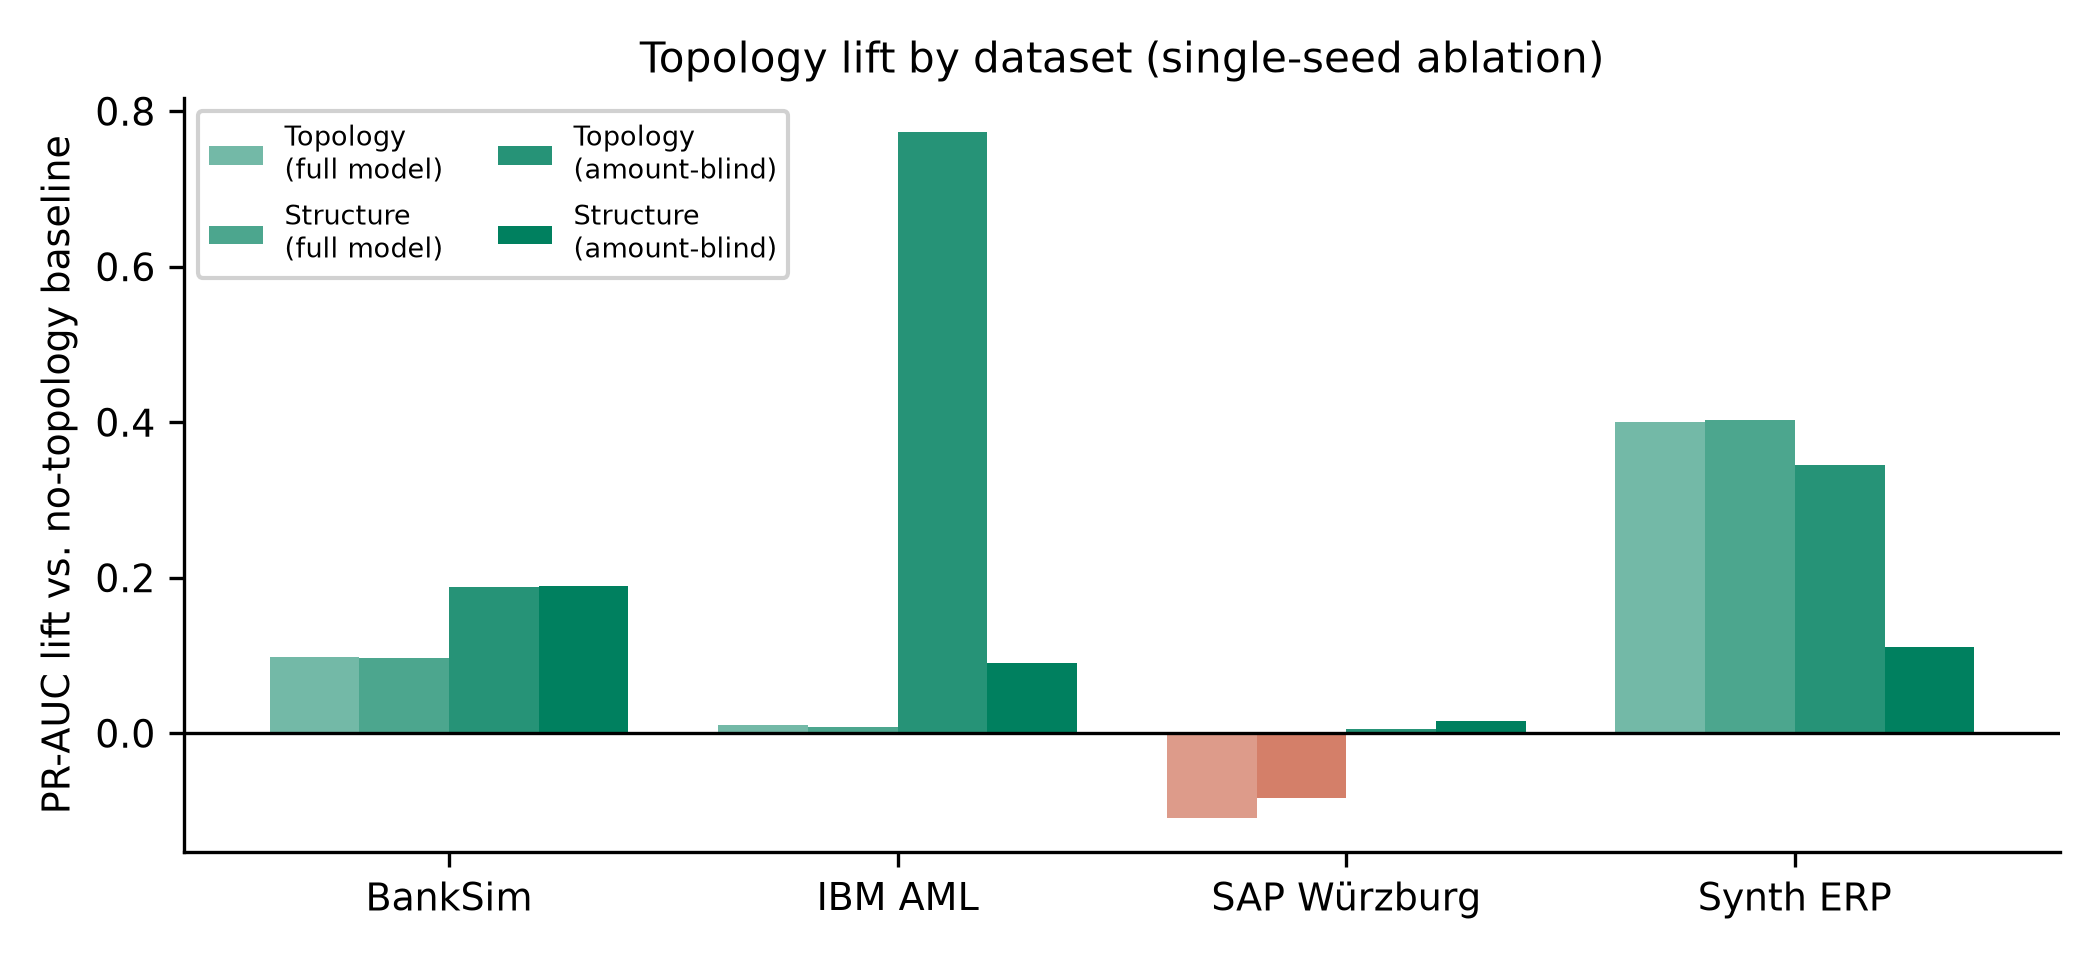
\includegraphics[width=\columnwidth]{figures/ablation_lift_by_dataset.png}
\caption{The four lift statistics of Table~\ref{tab:ablation-lifts} plotted by dataset, making visually explicit that SAP W\"urzburg is the only dataset where both full-model lifts are negative while its two amount-blind lifts remain (barely) positive.}
\label{fig:ablation-lift-by-dataset}
\end{figure}

\subsection{Dataset-by-dataset verdict}
\textbf{BankSim: yes.} The full-model structure lift is $+0.0974$ PR-AUC (an $11.7\%$ relative improvement over the $0.833$ baseline, $0.0974/0.833$), and — decisively — the clean amount-blind probe confirms it independently: with every amount feature removed from both sides of the comparison, pure structure still adds $+0.1899$ PR-AUC ($0.634 \to 0.824$). BankSim's topology-importance breakdown (\texttt{ablation.json}) attributes this almost entirely to two density features, \texttt{dest\_in\_degree} (gain importance $0.520$) and \texttt{fan\_in} ($0.091$): BankSim transactions run customer $\to$ merchant, so cycles are structurally impossible, and the signal that remains is exactly the "many senders funnel into one receiver" mule-collection pattern the fan-in features are built to detect. This is the cleanest positive result in the ablation, on a real (simulated-but-not-synthetic-generated) dataset, under both the contaminated and the clean test.

\textbf{IBM~AML: uninformative in the full model; the real signal is elsewhere.} The ordinary baseline alone already reaches PR-AUC $0.990$, leaving essentially no headroom: the full-model structure lift of $+0.0079$ is small in both absolute and relative terms, and — as \S\ref{sec:ablation-stats} makes explicit — falls below this project's own single-seed noise floor, so it cannot be read as evidence of anything. The dirty amount-blind topology probe reaches a striking PR-AUC of $0.867$ ($+0.7735$ lift over the amount-blind baseline's $0.093$), but this number is not evidence for structure: \texttt{topology\_importance} shows \texttt{lap\_out\_recur} ($0.540$) and \texttt{lap\_out\_payees} ($0.420$) together account for $96\%$ of the gain inside that arm, and both are the amount-derived lapping features excluded from the pure-structure set. The clean amount-blind structure probe — the only honest version of this test — reaches PR-AUC $0.184$, a lift of $+0.0905$ over the $0.093$ amount-blind baseline: real, but an order of magnitude smaller than the $0.867$ figure a less careful ablation would have reported as "topology's contribution." In short: IBM~AML's frauds are given away by recurring near-equal amounts (a re-encoded amount signal, not a graph shape), a finding this project's own earlier probing flagged as refuting its initial premise that IBM~AML would be the decisive topology testbed.

\textbf{SAP W\"urzburg: no — topology actively hurts.} Both full-model lifts are negative: $-0.1090$ for all topology, $-0.0829$ for pure structure alone (\texttt{marginal\_structure\_lift = -0.08288}, the number this project's own methodology rules single out as never to be softened or omitted). Adding any topology columns to the ordinary baseline drives test PR-AUC down from $0.155$ to $0.072$ (structure) or $0.046$ (all topology) — a genuinely negative result, not merely a null one. The two amount-blind lifts are small and positive ($+0.0056$, $+0.0153$), but both baselines they are measured against are themselves extremely weak (PR-AUC $0.049$), so this offers no rehabilitation. SAP W\"urzburg is also the one dataset in this study with only $25$ test-split frauds, which we treat as a hard interpretability ceiling rather than a footnote: with that few positive examples, a handful of ranking swaps can move PR-AUC by tens of a point, and \S\ref{sec:ablation-stats} presents an independent, multi-seed confirmation that this dataset's metrics are indeed unstable. We report the negative result plainly rather than either suppressing it or explaining it away, while being explicit that "topology hurts here" and "this measurement is high-variance" are both true simultaneously.

\textbf{Synth-ERP: yes, the largest lift measured — and the one result that cannot be used as thesis evidence.} The full-model structure lift is $+0.4031$ PR-AUC, a $246.8\%$ relative improvement over a weak $0.163$ baseline, with a clean amount-blind confirmation of $+0.1115$. This is real signal by every measure this ablation applies. It is also, definitionally, the least informative result for the paper's actual scientific claim: synth\_erp is this project's own generated dataset, built and calibrated specifically to have rich, ERP-flavored graph structure, and the project's binding policy (adopted precisely to avoid grading its own homework) treats it as a training/stress-testing corpus only, never as evidence that topology helps on real transaction data. We report the number because it is honest and instructive about what topology \emph{can} do when a dataset is constructed to contain strong structural fraud signatures — but it answers a different, narrower question than the one this section opened with.

\subsection{Statistical caveats: one seed, no confidence intervals, and a stated noise floor}\label{sec:ablation-stats}
Every number in Tables~\ref{tab:ablation-arms} and \ref{tab:ablation-lifts} comes from a single training run per arm (seed 42), not an average over repeated runs. \texttt{ablation.json} carries no standard deviations, no confidence intervals, and no significance tests, and none should be inferred from it. This project's own training harness documents its rationale for treating small single-seed margins with suspicion: per the comment in \texttt{src/modeling/harness.py}, "single-seed differences of $\sim$0.01 PR-AUC are within XGBoost's subsample noise," and \texttt{experiments/ablation.py}'s own verdict logic uses exactly this $0.01$ figure as the cutoff below which a lift is characterized as "adds $\sim$nothing" rather than a genuine effect. By this project's own stated standard, IBM~AML's full-model structure lift of $+0.00792$ is below the noise floor and is not distinguishable from zero on the evidence of a single seed — a second, independent reason (beyond baseline saturation) that the IBM~AML full-model comparison cannot be read as informative.

A separate, multi-seed experiment offers some corroborating context, though it is not a like-for-like repetition of the arms above: \texttt{final\_champions.json} trains each dataset's final champion configuration — ordinary $+$ topology $+$ TGN embeddings, a superset of the ablation's \emph{+Structure} arm that additionally includes the 65-dimensional temporal-graph-network features discussed elsewhere in this paper — three times, with seeds $\{42,43,44\}$, and reports mean $\pm$ standard deviation. Its per-dataset stability is informative about exactly the concern raised above: BankSim's three-seed test PR-AUC is $0.9364 \pm 0.0015$ (a $0.16\%$ relative standard deviation), consistent with this dataset's ranking being robust to seed choice; SAP W\"urzburg's is $0.1557 \pm 0.0717$ — a $46\%$ relative standard deviation on the mean — which independently corroborates, from a completely different experiment and feature set, the instability that the ablation's own 25-test-fraud caveat already predicts. SAP W\"urzburg's imbalance-mechanism selection for this same champion run is explicitly flagged \texttt{reliable:~false}, and its hyperparameter search was skipped altogether (validation frauds below the guard threshold described in \S\ref{sec:protocol}), so its champion runs on the harness's locked default configuration rather than a tuned one. None of this changes the ablation's central negative finding for SAP W\"urzburg — if anything it strengthens the case for treating that finding as directionally real but numerically imprecise, exactly as reported above — but it is a materially different, TGN-inclusive experiment and its numbers should not be conflated with the seed-42-only ablation arms in Tables~\ref{tab:ablation-arms}--\ref{tab:ablation-lifts}. We also note, to keep every PR-AUC in this paper unambiguous: the champion figures cited in this paragraph describe the offline, research-only model family evaluated for this ablation and are not the model served by the production audit console, which for latency and reproducibility reasons excludes the TGN component; that distinction is maintained precisely wherever this paper reports a PR-AUC for a specific model.

\subsection{The cycle-feature paradox}
The project's topology engine was built around five detectors intended to be its signature contribution — \texttt{in\_cycle}, \texttt{cycle\_length}, \texttt{in\_cycle\_ge3}, \texttt{cycle\_amount\_ratio}, and \texttt{cycle\_time\_span} — measuring whether a transaction closes a money loop, how long that loop is, and how tightly it conserves the amount that entered it. The ablation's own gain-importance breakdown does not support these as the load-bearing signal. Table~\ref{tab:cycle-importance} sums the gain importance of all five cycle features, within the full \emph{+Topology} model, against the single highest-importance density feature on the same dataset. On three of the four datasets — BankSim, IBM~AML, and SAP W\"urzburg — every one of the five cycle features scores exactly $0.0$ gain importance; the model finds no split in five hundred boosting rounds for which distinguishing "closes a 3-hop cycle" from "does not" reduces loss more than an already-available split on in-degree, fan-in, or (on IBM~AML) the amount-derived lapping columns. Only on synth\_erp — the one dataset engineered specifically to contain rich cyclic laundering structure — do the cycle features register non-zero importance, and even there their combined mass ($0.0275$) is roughly a third of the single top feature, \texttt{src\_out\_degree} ($0.0786$).

\begin{table}[t]
\centering
\caption{Combined gain importance of the five cycle features vs.\ the single highest-importance density feature, within the baseline+topology model. \texttt{topology\_importance}, \texttt{paper/data/ablation.json}.}
\label{tab:cycle-importance}
\small
\begin{tabular}{lccc}
\toprule
Dataset & $\Sigma$ cycle feats. & Top non-cycle feat. & Importance \\
\midrule
BankSim & 0.0000 & \texttt{dest\_in\_degree} & 0.5199 \\
IBM AML & 0.0018 & \texttt{lap\_out\_recur}$^\dagger$ & 0.5397 \\
SAP W. & 0.0000 & \texttt{fan\_in} & 0.1791 \\
Synth-ERP & 0.0275 & \texttt{src\_out\_degree} & 0.0786 \\
\bottomrule
\end{tabular}
\\[3pt]
\raggedright{\scriptsize $^\dagger$Amount-derived, not pure structure. Among pure-structure features on IBM AML, the top scorer is \texttt{dest\_in\_degree}/\texttt{fan\_in} at $0.0003$.}
\end{table}

%% FIGURE TODO: small-multiples heatmap, one panel per dataset, rows = the 13 topology feature names (grouped visually into the 8 pure-structure and 5 amount-derived features), single column of cell shading by gain importance value from topology_importance in ablation.json, making the "cycle features are a near-empty column on 3 of 4 panels" pattern visible at a glance.
\begin{figure}[t]
\centering
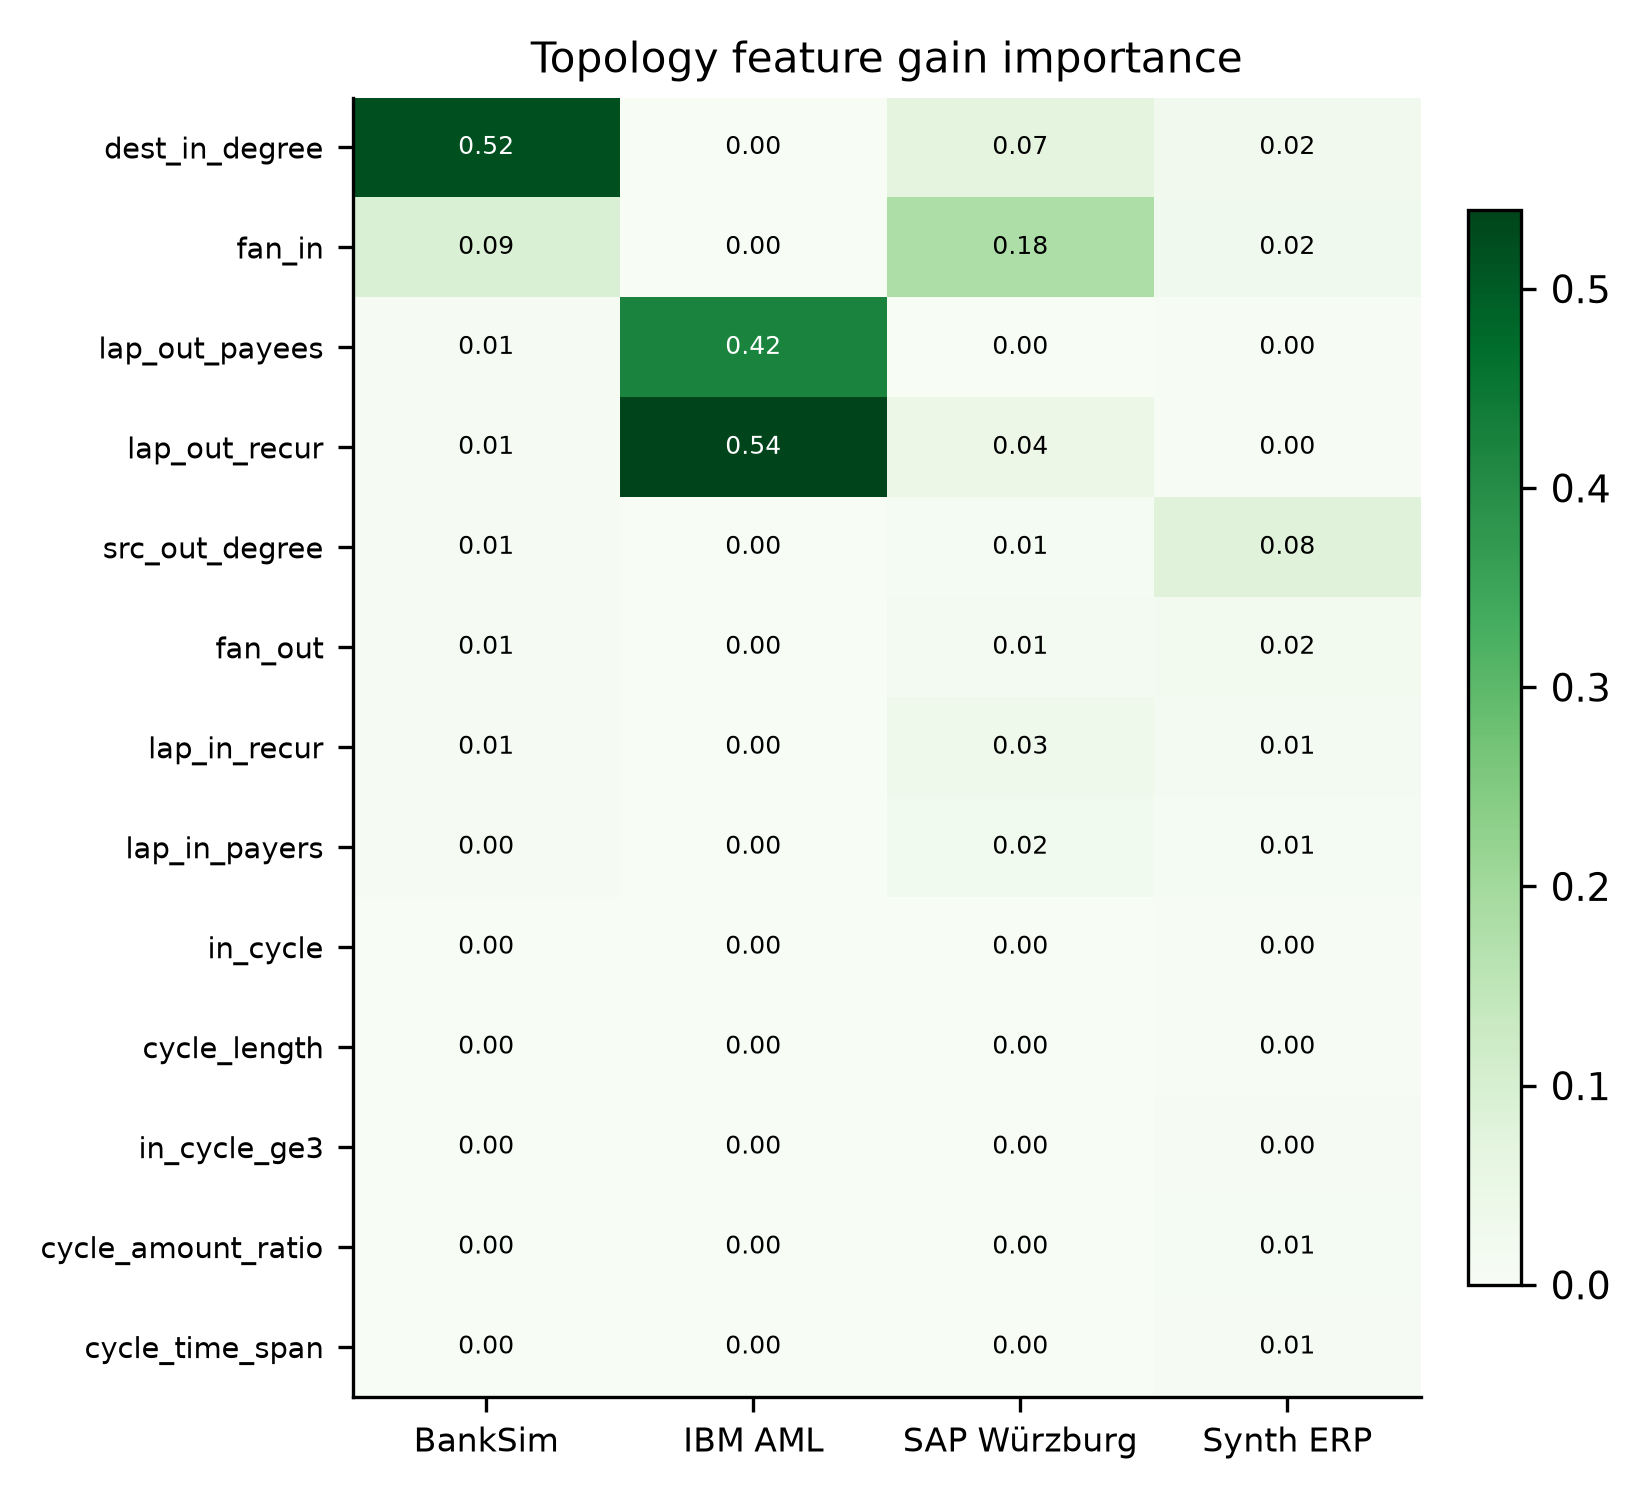
\includegraphics[width=\columnwidth]{figures/topology_importance_heatmap.png}
\caption{Topology feature gain importance by dataset (\texttt{topology\_importance}, Table~\ref{tab:cycle-importance}'s underlying data), grouping pure-structure against amount-derived features and making visible how consistently the five cycle features sit at or near zero while a small number of density features (in-degree, fan-in) or amount-derived lapping features carry essentially all of the mass.}
\label{fig:cycle-heatmap}
\end{figure}

This result should be read carefully rather than as "cycles carry no fraud signal." The topology-only arm of Table~\ref{tab:ablation-arms} shows the full thirteen-feature topology block, cycle features included, carries genuine standalone predictive power on every dataset (PR-AUC $0.483$, $0.633$, $0.024$, and $0.306$ respectively — all comfortably above the base rate for a heavily imbalanced problem). Gain importance measures a feature's marginal contribution to loss reduction \emph{inside a specific ensemble that already contains other features}, not its information content in isolation; a feature can be highly informative and still be assigned near-zero credit if a cheaper, earlier split on a correlated feature already captures most of the same discriminative power. That is the more precise version of the finding: on this project's own datasets, the density features (in-degree, fan-in) and, where present, amount-derived lapping features are close enough substitutes for "this transaction closes a laundering loop" that the boosted-tree ensemble routes around the cycle detectors almost entirely, even after this project's own earlier work deliberately upgraded the cycle detector to be more discriminative (amount-conservation ratio, loop tightness, a $\geq$3-hop flag) specifically to address a similar finding in the project's predecessor codebase. The cycle detectors remain part of the shipped feature set — they are, as later sections of this paper discuss, considerably better human-facing evidence for an auditor than "high in-degree" is — but the ablation does not support treating them as this project's primary source of predictive lift. That role, on the evidence gathered here, belongs to simple connectivity density.